\begin{frame}[t]{Модел на Hindmarsh-Rose}
    Модел на Hindmarsh-Rose е обезразмерена система от 3 ОДУ, 
    като на трансмембранния потенциал съпоставим $x$,
    а $y$ и $z$ съответстват на преминаване на йони през мембраната.
    \begin{align*}
        &\dv{x}{t}=y + \varphi(x) - z + I\\
        &\dv{y}{t}=\psi(x) - y\\
        &\dv{z}{t}=r\left(sx - sx_R - z\right)
    \end{align*}
    Функциите $\varphi$ и $\psi$ съответстват действието на помпите и се изразяват:
    \begin{align*}
        &\varphi(x) = -ax^3 + bx^2\\
        &\psi(x) = c - dx^2
    \end{align*}
\end{frame}

\begin{frame}[t]{Модел на Hindmarsh-Rose}
    Общо имаме 8 параметъра. Очаквано, динамиката на модела е разновидна, зависимост от избора на стойностите им.
    Въпреки това, самият модел не е сложен от изчислителна гледна точка.
    \begin{figure}[htbp!]
        \centering
        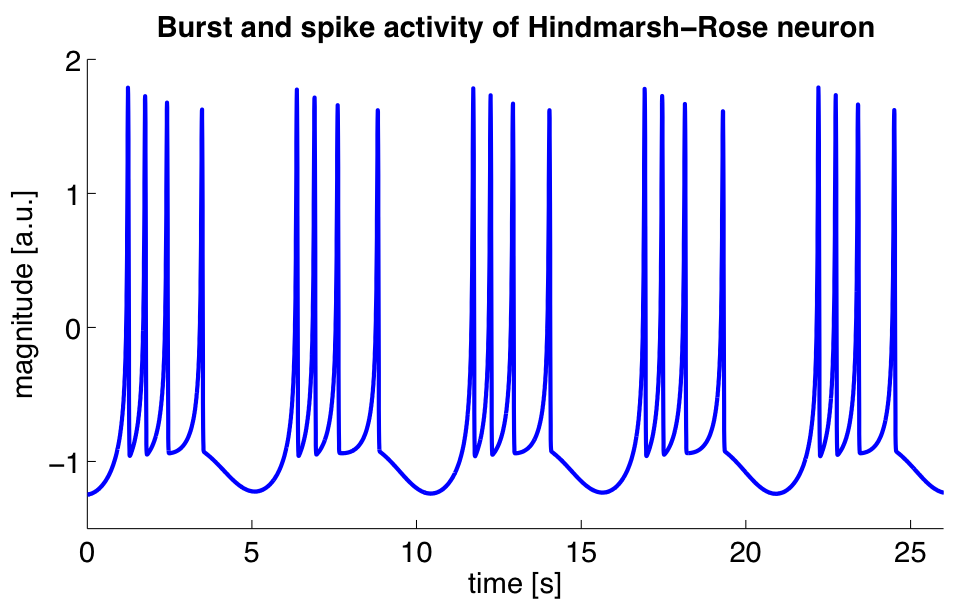
\includegraphics[width=\textwidth,height=0.7\textheight,keepaspectratio]{hindmarsch-rose-graph.png}
        \caption{Симулация на модела от Wikipedia}
    \end{figure}  
\end{frame}